\section{Konzeption einer an den spezifischen Workflow angepassten Anwendung}

Im Abschnitt~\ref{l:problemanalyse} ab Seite~\pageref{l:problemanalyse} ff. wurde analysiert, welche Probleme in Zusammenhang mit der Produktion von Informations- und Kommunikationsmedien bezüglich den verwendeten Texten entstehen, wenn Textverarbeitungs- und Tabellenkalkulationsprogramme wie \emph{Microsoft} \emph{Word} und \emph{Excel} verwendet werden. Aus dieser Analyse wird in diesem Abschnitt das Konzept für eine Anwendung entwickelt, die den Workflow mit allen Beteiligten und deren Anforderungen abbildet. Hierzu werden in Abschnitt~\ref{l:workflow} zuerst die Arbeitsabläufe in Projekten analysiert. Zusammen mit der Schlussfolgerungen aus dem vorangegangenen Kapitel werden dann in Abschnitt~\ref{l:anforderungen} die Anforderungen an eine Lösung beschrieben. 

% MARK

\subsection{Der spezifische Workflow}\label{l:workflow}

Beobachtet man verschiedene Projekte, in denen Informations- und Kommunikationsmedien erstellt werden, lässt sich feststellen, dass Texte immer wieder auf die gleiche Art beeinflusst werden. Für eine vollständige Beschreibung des Workflows ist es zunächst sinnvoll, zu ermitteln, \emph{wie} Texte beeinflusst werden. 

% MARK

\begin{figure}[htb]
\begin{center}

\includegraphics[width=\textwidth]{media/chart-3.pdf}
\end{center}
\caption{Operationen bei der Erstellung von Texten}
\label{chart:3}
\end{figure}

Betrachtet man die Arbeiten in Zusammenhang mit Text lassen sich diese in sechs eigenständige Operationen unterteilen:

\begin{enumerate}
\item{Durch \textbf{Definieren eines Textbausteines} wird festgelegt, wie der benötigte Text beschaffen sein muss. Die Aussage \typoquotes{Wir brauchen an dieser Stelle eine Überschrift} ist ein Beispiel für diese Operation. Sie legt fest, wie der Textbausteine gestaltet werden muss, um die ihm zugedachte Aufgabe zu erfüllen. Neben der Angabe zur Platzierung auf dem Medium durch \typoquotes{an dieser Stelle} wird implizit durch \typoquotes{eine Überschrift} eine Angabe zur inhaltlichen und visuellen Gestaltung getroffen; Überschriften sollen kurz und knapp sein und ihre visuelle Gestaltung wird durch den Styleguide des Projektes festgelegt.}
\item{Das \textbf{Schreiben eines Textes} befüllt einen Textbaustein mit einem Text in einer Sprache. Bei diesem Vorgang wird der Text entsprechend der Vorgabe aus der Beschreibung als Original erstellt oder aus Quellen außerhalb des Projektes kopiert und eingefügt. }
\item{In der \textbf{Korrektur} wird der Text inhaltlich und grammatikalisch überprüft und entsprechend angepasst. Der Korrektor muss dabei für eine grammatikalische Überprüfung des Textes kein Fachwissen bezogen auf das Projekt haben. Ist diese Fachwissen vorhanden, kann eine inhaltliche Korrektur vorgenommen werden.}
\item{In der \textbf{Qualitätskontrolle} wird der Text dahingehend überprüft, ob er den Anforderungen gemäß der Beschreibung und inhaltlichen Vorgaben, auch hinsichtlich des gesamten Projektes entspricht. }
\item{Durch die \textbf{Freigabe} wird der Text abgenommen und kann nun in das Endprodukt übernommen werden.}
\item{Durch die \textbf{Veröffentlichung} wird der Text in das Endprodukt eingebracht.}
\end{enumerate}

\begin{figure}[htb]
\begin{center}
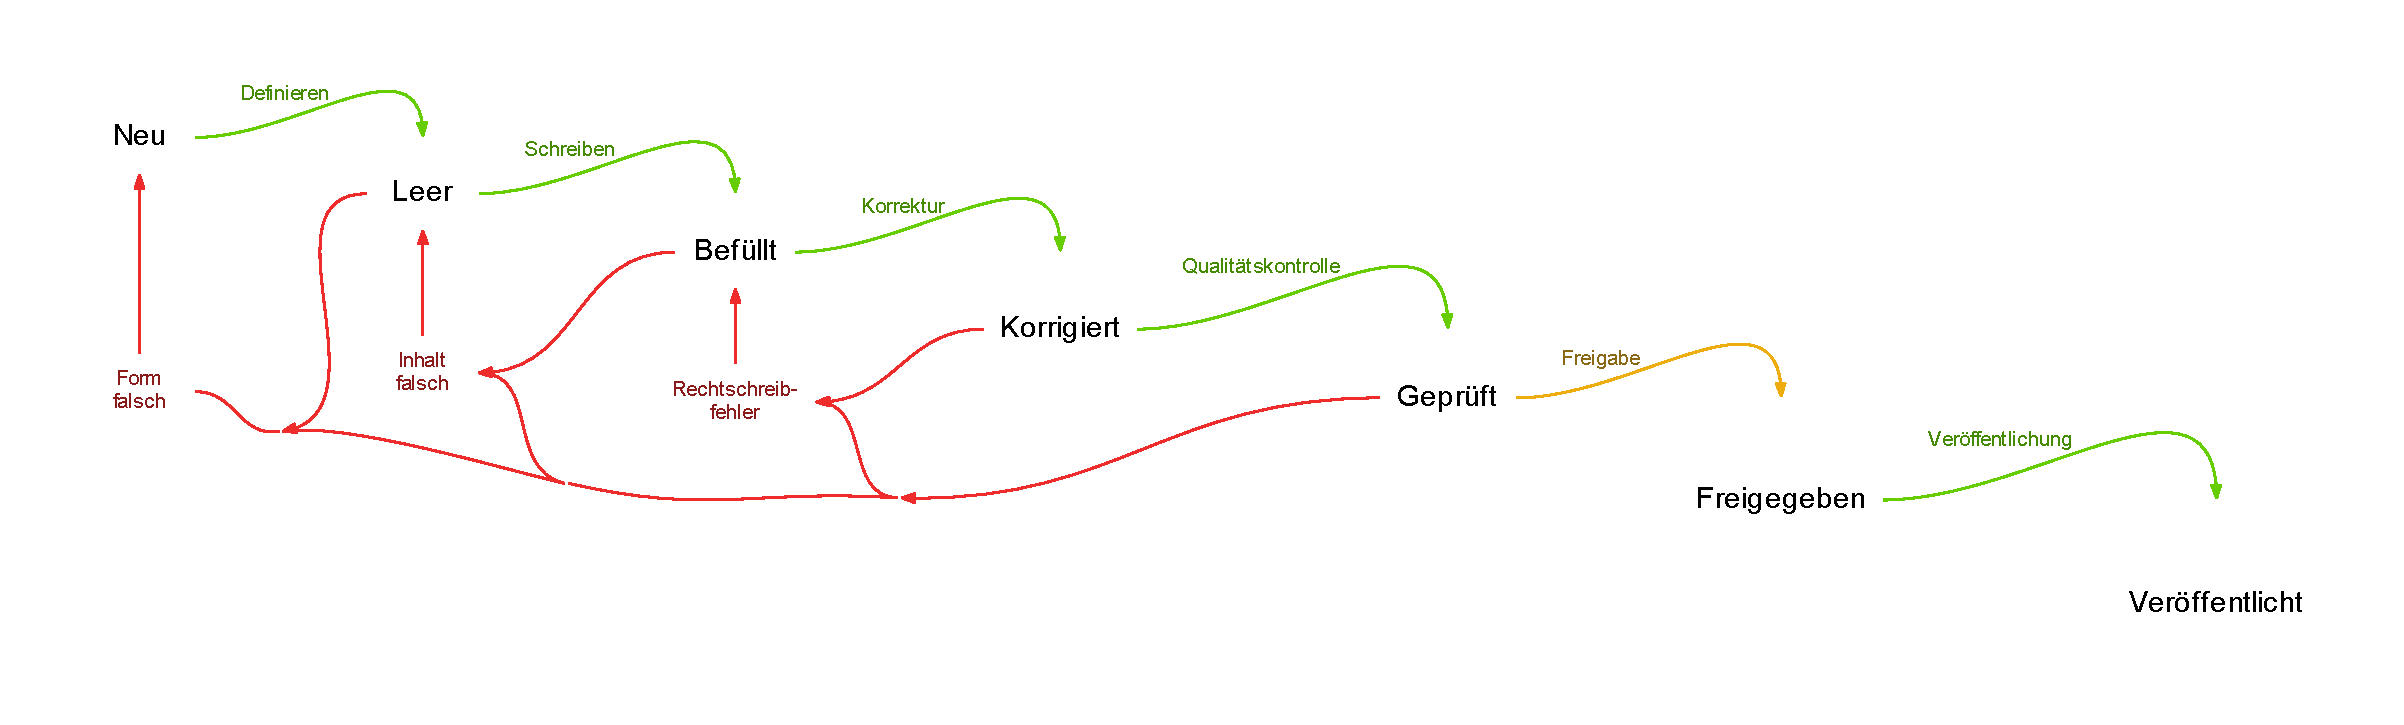
\includegraphics[width=\textwidth]{media/chart-4.pdf}
\end{center}
\caption{Operationen bei der Erstellung von Texten mit Qualitätskontrolle}
\label{chart:4}
\end{figure}

Diese Operationen werden auch 1:1 auf die übersetzte Version eines Textes angewendet.

\begin{figure}[htb]
\begin{center}
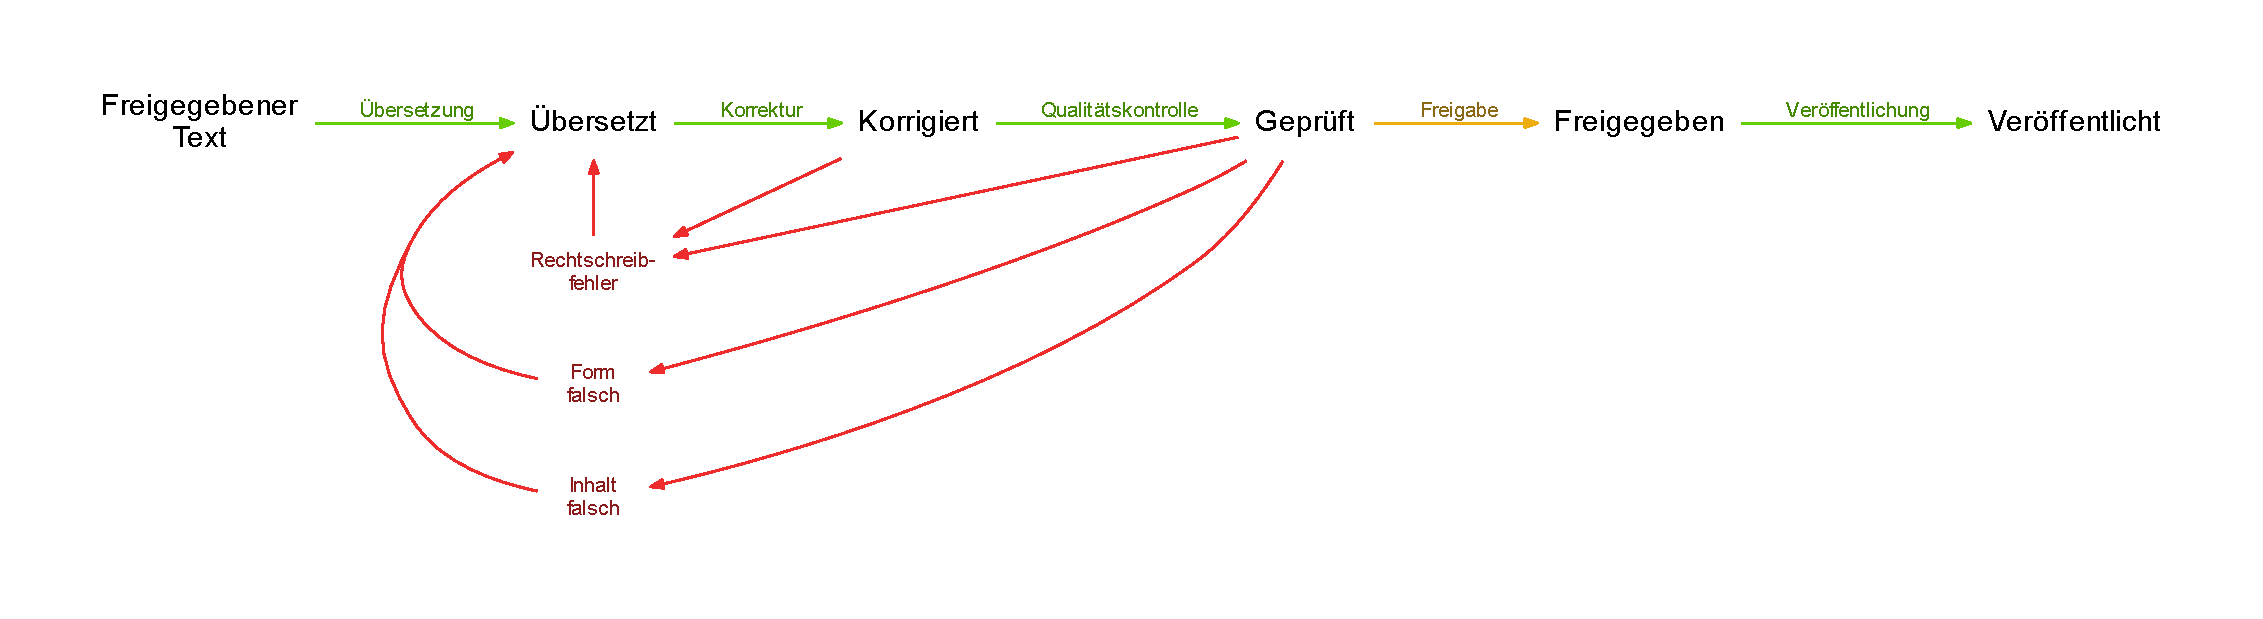
\includegraphics[width=\textwidth]{media/chart-5.pdf}
\end{center}
\caption{Operationen bei der Übersetzung von Texten mit Qualitätskontrolle}
\label{chart:5}
\end{figure}

In Abschnitt~\ref{l:besondererolle} ab Seite~\pageref{l:besondererolle} wurde beschrieben, wie umfangreich die Anzahl der Personen ist, die Einfluss auf die Texte eines Produktes haben. Die Rollenverteilung ist dabei von Projekt zu Projekt unterschiedlich. Allen gemeinsam ist aber, dass die beteiligten Personen  Einfluss auf drei grundlegenden Eigenschaften von Text haben: den Inhalt des Textes, die Attribute wie z.B. \typoquotes{maximale Textlänge} oder \typoquotes{Position im Medium} und den Status wie z.B. \typoquotes{neu} und \typoquotes{freigegeben}. Anhand dieses Kriteriums lassen sich Mitarbeiter in drei Gruppen unterteilen:

% MARK

\paragraph{Personen, die Einfluss auf den Inhalt haben}

\paragraph{Personen, die Einfluss auf den Attribute haben}

\paragraph{Personen, die Einfluss auf den Status haben}




\begin{enumerate}
\item{Der \textbf{Informationsarchitekt} (oder Konzepter) legt die Struktur eines Produktes fest und damit auch die Art und Menge des benötigten Textes,}
\item{der \textbf{Texter} verfasst die Texte,}
\item{der \textbf{Übersetzer} überträgt die Texte in weitere Sprachen,}
\item{der \textbf{Qualitätsmanager} überwacht die Ergebnisse der Prozesse,}
\item{der \textbf{Produktbesitzer} (oder Kunde) ist für die fachlichen und rechtliche Aspekte, sowie das Festlegen der zeitlichen Rahmenbedingungen verantwortlich,}
\item{der \textbf{Produzent} ist für die Erstellung des eigentlichen Produktes verantwortlich.}
\end{enumerate}

Alle Rollen haben im Verlauf eines Projekts, zu unterschiedlichen Zeiten und mit unterschiedlichem Gewicht, Einfluss auf die Gestaltung der Texte. Es existieren auch Abhängigkeiten zwischen den Rollen, so kann ein Übersetzer erst arbeiten, wenn der Text vorliegt und vom Produktbesitzer abgenommen wurde; wird aber zu einem späteren Zeitpunkt der Text geändert, muss auch wieder der Übersetzer neu beginnen.

\subsection{Anforderungen}\label{l:anforderungen}

Wie in der Schlussfolgerung in Abschnitt~\ref{l:schlussfolgerung} bereits erwähnt ergeben sich aus den genannten Problemen im vorangegangenen Kapitel die folgenden Anforderungen an eine Lösung.

\paragraph{Gleichzeitiges Bearbeiten von Texten} Es soll möglich sein, dass alle  Mitarbeiter gleichzeitig an den Texten eines Produktes arbeiten.



\subsection{Eigenschaften von Texten}
\label{l:textattribute}

\paragraph{Typ} Überschrift, Untertitel, Bild-Beschreibung, Fließtext.

\subsection{Beschreibung der notwendigen Funktionalität}

Unterteilung in Muss- und Kann-Kriterien

\subsection{Nachteile/Risiken des Konzepts}

\subsection{Funktionale Anforderungen}

\label{l:anforderungen}

\TODO

Aufteilen der Texte in einzelne Bausteine um diese eindeutig identifizieren zu können. Dies verhindert Copy\&Paste-Fehler (vgl. S.~\pageref{p:serielles-konzept}).

\label{l:hierarchien} Hierarchien sind aber in allen Produkten vorhanden und ein natürlicher Weg, Informationen zu gliedern. 




